\documentclass[pdftex,a4paper,titlepage,11pt,openright]{article}
\usepackage[T1]{fontenc}
\usepackage[utf8]{inputenc}
\usepackage[english,francais]{babel}
\usepackage{listings}
\usepackage{setspace}

\usepackage{avant}
\usepackage{fancyvrb}
\usepackage{fancyhdr}
\pagestyle{fancy}
\fancyhf{}
\fancyhead[LE,RO]{\itshape\thepage}
% \fancyhead[LO]{\itshape\rightmark}
% \fancyhead[RE]{\itshape\leftmark}
\renewcommand{\headrulewidth}{0.5pt}
\usepackage[top=2.5cm, bottom=2.5cm, left=3.0cm, right=3.0cm, a4paper]{geometry}
% \addtolength{\headheight}{0.5pt}
% \renewcommand\footrulewidth{0pt}
\fancypagestyle{plain}{
    \fancyhead{}
    \renewcommand{\headrulewidth}{0pt}}
\usepackage{textcomp}
\usepackage{relsize}
\usepackage{amssymb}
\usepackage[colorlinks=true,linkcolor=black,citecolor=black,urlcolor=black,filecolor=black]{hyperref}
\usepackage{framed}
\usepackage[pdftex]{graphicx}
\usepackage{makeidx}
% \addtolength{\textwidth}{1cm}
% \setlength{\textheight}{24cm} 	% Hauteur de la zone de texte


% nouvelle commande pour un joli nom
\newcommand{\nom}[1]{\textsc{#1}}

% commande pour une zolie ligne
\newcommand{\ligne}[1][1pt]{
  \par\noindent
  \rule[.5ex]{\linewidth}{#1}\par}

% nettoyer une page blanche avant une page de chapitre en mode openright
\newcommand{\clearemptydoublepage}{
	\newpage{\pagestyle{empty}\cleardoublepage}}


\makeindex

\begin{document}

% augmenter l'espacement entre plusieurs paragraphes plutôt que de passer des lignes quand il faut pas
\setlength{\parskip}{2.4ex}

\title{
\ligne{\Large}
\textbf{Audit Security}\\
\textbf{Project de deuxième année}\\
\Large Capture d'activité système pour PIGA-SYSTRANS
% \Large Généralisation des plugins de communication avec contextd
\ligne{\Large}
}
\author{\nom{Dimitri Gressin} \& \nom{Timothée Ravier}\\\\\nom{Pilote : Jérémy Briffaut}}
\date{20 \textsc{janvier} 2011} %TODO

% titre
\maketitle

% page blanche
\clearemptydoublepage

% table des matières
\setcounter{secnumdepth}{2}
\setcounter{tocdepth}{2}
\addtocontents{toc}{\protect\thispagestyle{empty}}
\tableofcontents
\addtocounter{page}{-1}

\newpage

\section*{Introduction} \addcontentsline{toc}{section}{Introduction}
Ce rapport présente le travail et les résultats obtenus à la fin du premier semestre, dans le cadre de notre projet d'application de deuxième année.
%TODO

~

Le but de ce projet est de généraliser la communication entre les différentes applications et le daemon contextd. Contextd permet 
%TODO
Jusqu'à présent, la communication entre les applications et contextd s'effectuait via un pluging ou un patch propre à chaque application. Contextd recueil alors les différentes opérations qu'elles effectuent (lecture/écriture de fichiers, création de socket, etc.) pour en déduire un contexte. En effet, il est pour l'instant nécessaire de modifier chaque application pour lui permettre de valider ses actions avec contextd. L'idée retenue consiste à déplacer la contrainte de communication au niveau du noyau, qui par l'intermédiaire des appels systèmes a connaissance des actions entreprises par les programmes.
%TODO

~

\section*{Objectifs} \addcontentsline{toc}{section}{Objectifs}

Pour pouvoir se séparer des plugins/modifications par applications, il est nécessaire de communiquer à contextd certaines informations sur le comportement des programmes. Il faut notamment obtenir :
\begin{itemize}
	\item la liste des fichiers créés, ouverts, modifiés par l'ensemble des processus, et les contextes SELinux associés, si le module SELinux est activé.
	\item la liste des connexions ouvertes par le systeme, et plus particulièrement les adresses IP de destination, et donc finalement le nom de domaine de destination.\\
\end{itemize}

De plus, il faut que le programme puisse attendre la réponse de contextd avant de poursuivre son exécution.

\newpage





\section{Systemtap}

\subsection{Principe de fonctionnement}

Nous avons ainsi commencer par utiliser Systemtap, un outil d'analyse du noyau grâce à des scripts qui ne nécessite pas de modifier le code du noyau. Systemtap utilise les KProbes, et les Kretprobes\cite{IBMRBST} pour intervenir à différents endroits dans le déroulement des fonctions du noyau pour permettre à l'utilisateur de lire certaines variables ou de logger certains appels système. Le principe de fonctionnement de Systemtap est résumé sur le schéma ci-dessous.

\begin{figure}[hb]
	\centering
	\includegraphics[scale=0.4]{kretprob.png}
	\caption{Fonctionnement tel que décrit dans la référence IBM sur Systemtap \cite{IBMRBST}}
\end{figure}

\newpage

\subsection{Résultats obtenus}

Après s'être familiarisé avec le fonctionnement de Systemtap, nous nous sommes aperçu que les scripts utilisés pour récupérer les informations issues des appels système sont exécutés une fois l'appel système effectué. Il n'est pas possible, d'après nos recherches, de faire en sorte que les scripts puissent bloquer les appels systèmes avant de les effectués.

De ce fait, l'utilisation de Systemtap ne permet pas de répondre à nos besoins.

Il faut ajouter à cela que les informations recueillies à partir de Systemtap ne sont pas exploitables pour certaines d'entre-elles. Par exemple, lorsqu'un fichier est accédé (lu ou écrit), seul le numéro d'inode nous était retourné. Il n'était alors pas pertinent de récupérer le chemin complet du fichier, car cette recherche est inadapté et inefficace : il est nécessaire de parcourir l'intégralité du système de fichiers.

Il fallait donc changer de stratégie. C'est pourquoi, nous avons, avec l'accord du responsable du projet, Jérémy Briffaut, décidé de nous orienter vers l'utilisation des ``Linux Security Modules'' (LSM).

\newpage

\section{Linux Security Modules}

\subsection{Principe de fonctionnement}

Les modules LSM sont au noyau ce que netfilter est au réseau.

Le principe de fonctionnement est simple : un module LSM est chargé dans le noyau Linux au démarrage. Il se substitue ou complète alors la procédure de contrôle d'accès. \`A chaque appel système est associé un hook que l'on peut considérer comme une fonction. Il est placé dans l'appel système entre les vérifications élémentaires (existence des fichiers, droits unix) et sa réalisation. Dès qu'un appel système est demandé, le hook est exécuté. Par défaut, il autorise l'exécution de l'appel système.

\begin{figure}[hb]
	\centering
	\includegraphics[scale=0.45]{lsm1.png}
	\caption{Architecture des hooks LSM \cite{LSMINTRO}}
\end{figure}

L'avantage de ces hooks est qu'ils offrent une très grande liberté. Cependant, il n'est possible pour le moment que de charger dans le noyau qu'un seul et unique module LSM. Or, PIGA utilise déjà un module LSM modifié, celui de SELinux.

Pour simplifier le développement, nous avons désactivé SELinux. \`A terme, il se pourrait que SELinux soit définitivement désactivé.

\begin{figure}%[hb]
	\centering
	\includegraphics[scale=0.45]{lsm2.png}
	\caption{Hook LSM permissif. Ce hook autorise la politique de sécurité à passer outre les restrictions DAC \cite{LSMINTRO}}
\end{figure}

\newpage

\subsection{Ce qui a été réalisé}

Nous avons donc développé un module LSM qui "hook" les appels systèmes. Par défaut, ces hooks sont "transparents" à l'exception du hook "file permission" sur lequel nous travaillons. Il est appelé à chaque ouverture (lecture, écriture, exécution) de descripteur de fichier.

Par la suite, il faudra convenir des appels systèmes sur lesquels il est intéressant d'intervenir.

Nous avons ajouté la possibilité d'activer ou non ce module lors de la compilation du noyau en suivant les conventions de nommage des options de configuration.

Ensuite, nous avons commencé à chercher les différentes informations nécessaires à contextd pour son fonctionnement, et plus particulièrement ce qui concerne le hook "file permission" :
	\begin{itemize}
		\item le PID
		\item l'execname
		\item le chemin complet du fichier
		\item ...
	\end{itemize}

Nous avons également remarqué que le hook "socket bind" permet de récupérer des informations, notamment l'adresse IP et le port de destination d'une socket, avant qu'elle ne soit créée. Son fonctionnement doit être confirmé, car il pourrait nous affranchir d'utiliser une alternative telle que ULOG et iptables.
	\begin{itemize}
		\item[-] le PID
		\item[-] l'execname
		\item[-] la structure de la socket
		\item[-] L'adresse de connexion
		\item[-] ...
	\end{itemize}

La principal difficulté de cette étape était de localiser dans quels fichiers ses informations sont localisées dans l'ensemble du code source du noyau Linux.

L'étape suivante consiste à envoyer les informations récupérées dans l'espace noyau à l'espace utilisateur. Nous avons envisagé plusieurs pistes, pour l'instant restées infructueuses.

\newpage

\subsection{Idées abandonnées}

\subsubsection{Socket Unix}

Tout d'abord, nous avons essayé de créer une socket Unix pour communiquer avec l'espace utilisateur. Cependant, les sockets NETLINK ne garantissent pas que les informations sont correctement envoyées. Il devient alors difficile de maîtriser le comportement du hook : il n'y a donc aucune garantie quant à la poursuite ou non de l'appel système.

\subsubsection{Appels système}

Nous avons envisagé de créer trois nouveaux appels systèmes pour répondre au besoins de communications entre le noyau et contextd. Un appel système nous aurait permis de transmettre une structure où nous stockons toutes les informations nécessaires à contextd et de la transmettre. Cela nous évite ansi de parser des informations et donc de gagner du temps, resource essentielle vu que chaque appel système ralonge la durée entre la demande d'une application et la réponse finale du noyau.

\subsection{Prochain développements}

Création de 3 nouvels appels systèmes pour répondre au besoins de communications entre le noyau et contextd. Pourquoi un appel système plutôt qu'un device ou une fifo? il permet de remplir une structure où nous stockons toutes les informations nécessaires à contextd. Cela nous évite ansi de parser des informations et donc de gagner du temps, resource essentielle vu que chaque appel système ralonge la durée entre la demande d'une application et la réponse finale du noyau.

%TODO Schéma de principe de communication avec le noyau, le daemon, les appels systèmes, contextd.

Pour s'assurer que les communications ne vont pas se mélanger mais bien se dérouler dans l'ordre, nous avons utilisés des verrous au niveau du noyau. Il a donc était nécessaire de vérifier que la mise en place de ces verrous n'entrainait pas d'état bloquant indéfiniement.

\begin{figure}[hb]
	\centering
	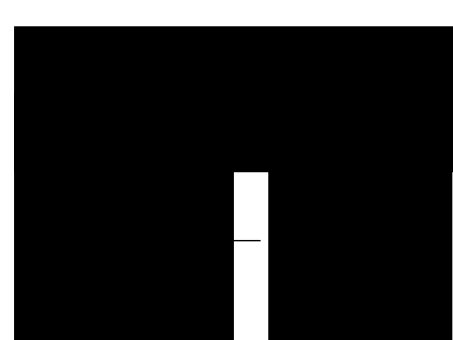
\includegraphics[scale=1]{syscall_sync.pdf}
	\caption{Communication entre les hooks LSM et les appels systèmes}
\end{figure}
%TODO Graphe d'états permettant d'assurer que les verrous dans les appels systèmes n'entrainent pas d'état bloquant sans sortie au niveau du noyau.

\newpage

\clearemptydoublepage

\section*{Conclusion} \addcontentsline{toc}{section}{Conclusion}

Le retard sur la partie implémentation noyau est principalement dûe à notre découverte très progressive des capacités offertes aux développeurs. Le livre Linux Kernel Development \cite{LKDSE} nous a permis de faire un bon en avant et d'implémenter les appels systèmes, ...

%Ce projet aura été pour nous l'occasion d'apprendre un langage de programmation orienté objets, qui nous a permis de gagner en efficacité lors de la phase de développement. En revanche, le fait que nous découvrions le C++ a limité nos possibilités d'optimisations. Le temps de traitement d'un graphe contenant une grande quantité de noeud étant élevé, il paraît nécessaire de paralléliser les algorithmes que nous avons appliqués, pour tirer pleinement partie des machines multi-coeurs ou multi-processeurs, par exemple en utilisant les Intel Threading Building Blocks \cite{IBMRBST}.

%De plus, bien que vérifiée, notre implémentation de l'algorithme de décomposition modulaire peut contenir des bugs. Il faut donc prévoir un outils permettant la vérification des résultats obtenus par cette méthode avec ceux obtenus par le parcours simple de graphes. Il sera donc toujours nécessaire de produire l'intégralité des chemins entre deux noeuds à partir du graphe d'origine pour s'assurer que les graphes réduits sont bien justes.

%Il faut noter, au vu des résultats, que la décomposition modulaire de graphes permettra fort probablement non seulement d'accélerer le parcours de graphes une fois l'intégralité des chemins générés mais aussi de réduire la taille finale de l'ensemble formé par tous les chemins.

%Enfin, notre programme se limite à la décomposition de graphes orientés. Les algorithmes diffèrent de ceux applicables aux graphes non-orientés et leur mise en oeuvre nécessiterai la réécriture d'une grande partie du code pour assurer la rapidité et l'efficacité de notre implémentation.


\newpage
\addcontentsline{toc}{section}{Annexes}
% \addcontentsline{toc}{subsection}{Remarques}
\addcontentsline{toc}{subsection}{Liens et références}
% \subsection*{Remarques}

%Un fichier de configuration est présent avec les sources du kernel 2.6.32-hardened. Il correspond aux options nécessaire à la compilation dans une machine virtuelle Virtualbox. L'option autorisant nos modifications y est aussi activée. Elle est situé dans Security -> SELinux userspace audit.

\subsection*{Liens et références}
\begin{thebibliography}{40}
\bibitem{IBMRBST} \textit{IBM Redbooks : SystemTap: Instrumenting the Linux Kernel for Analyzing Performance and Functional Problems}, \url{http://www.redbooks.ibm.com/abstracts/redp4469.html}

\bibitem{LSMINTRO} \textit{Linux Security Modules : General Security Support for the Linux Kernel}, \url{http://citeseerx.ist.psu.edu/viewdoc/download?doi=10.1.1.84.6867&rep=rep1&type=pdf}

\bibitem{SOURCE} Code source (kernel 2.6.32 hardened r9 et scripts systemtap) disponible sur le serveur de projet STI (le projet s'appelle pour l'instant ``Projet LSM''), \url{http://projetsti.ensi-bourges.fr/projects/promo2012-systemtap}.

\bibitem{LKDSE} \textit{Linux Kernel Development, Second Edition}, Robert Love, Novell Press
\end{thebibliography}

%\printindex

\end{document}
